\section{Description of \coolName}
\label{sec:description}

\TODO{Ici, je ne sais pas si onn peut beaucoup compresser, mais relire quand même}


Bringing everything together, we designed the stream cipher \coolName{}.
Its overall structure is presented in Section~\ref{sec:description-structure}, its details are explained in Section~\ref{sec:sepc-details}, and the influence of noise is discussed in Section~\ref{sec:rationale-controllin-noise}. A reference implementation can be found at
  \url{https://github.com/CryptoExperts/Transistor/}.

\subsection{Overall Structure}
\label{sec:description-structure}


\paragraph{Usage.}
\label{sec:usage}
%\lp{j'ai encore bidouillé cette partie, qu'en pensez-vous?}
\coolName{} is a stream cipher that generates a keystream consisting of elements from \( \mainField = \mathbb{F}_{17} \), referred to as {\em digits}.  It is intended for transciphering, i.e., for the type of protocol we summarized in the introduction\ifeprint (see Figure~\ref{fig:transciphering-principle})\fi.
More precisely, a 128-bit master key and an IV are used to initialize the internal state of \coolName{} using  a PRF (namely, {\tt SHAKE}~\cite{add:SHA3}), as suggested in~\cite{FSE:BerGil07}. This initialization  is only performed on the client side, and in particular is not evaluated homomorphically, meaning that its cost is negligible. On the other hand, it ensures for example that related IVs cannot be exploited. The entire resulting internal state is then encrypted using TFHE and sent alongside the ciphertext. This ciphertext is obtained by casting the plaintext message to a string of digits of $\mainField$, which is added digit by digit to the keystream produced by \coolName{} using the group law of $\mainField$.



% \ac{My two cents: Il faut qu'on dise clairement s'il y a une IV ou non. Plus je réfléchis, moins je trouve convaincant de dire qu'il n'y a pas d´IV, car cela veut dire qu'on tire une nouvelle clef au hasard à chaque msg. Ca n'est pas top, non ? Par contre, on peut dire que son coût n'est pas important, et donc qu'on peut choisir une initiation coûteuse, car elle n'est jamais faite côté serveur.}

  

%\lp{j'ai pensé parler ici de l'overhead impliqué par l'envoi de la clef maître mais en fait on en parle déjà et dans l'intro et dans les benchmarks...}

% \lp{@cryptoExperts: ça serait cool de remettre une couche ici sur le fait qu'on puisse choisir $p$ comme ça nous arrange, histoire qu'on ne se reprenne pas un reviewer chafouin persuadé que notre choix de $p$ nous condamne à l'inutilité}
% \nicolas{ajouté ci-dessous}
% \ac{Je pense que cette argumentation doit aller ailleurs, peut-etre ds la section précédente sur le choix de \(p\) mais pas ici.}
%\lp{j'ai gardé la toute première phrase de la discussion sur $p$ ici et j'ai bougé le reste de cette discussion plus haut, dans le paragraphe ``The parity of the plaintext space''}\yr{Modifié des trucs mineurs ici dans le paragraphe ci-dessus}


\paragraph{Internal State.}
The overall structure of \coolName{} is outlined in Figure~\ref{fig:structure}.

The idea is to generate two pseudo-random sequences with a very long
period using two distinct LFSRs. One of them generates whitening
subkeys, while the other acts as a sort of key schedule. The output of
the latter is fed into a Finite State Machine (FSM) with its own
state, and which operates on it using non-linear operations. We thus
have the following components:
\begin{itemize}
\item a register of 16 elements of $\mainField$ (the \emph{FSM state}),
\item an LFSR over $\mainField$ (the \emph{key schedule} or \emph{key-LFSR} $\pseudoKS$) of length $|\pseudoKS| = 64$, 
\item an LFSR over $\mainField$ (the \emph{whitening LFSR} $\whitening$), of length $|\whitening| = 32$,
\item a non-linear round function from $\mainField^{16}$ to itself (the \emph{round function}), and
\item a filter $\filter : \mainField^{16} \to \mainField^4$ that extracts $4$ digits from the FSM.
\end{itemize}

%\lp{j'ai rajouté le texte ci-dessous pour spécifier l'initialisation et le claim de sécurité.}

The FSM state is initialized to all zeros, and each LFSR is initialized using digits derived from the 128-bit master key and IV using SHAKE~\cite{add:SHA3}. 
\ifeprint
  We provide a detailed algorithm in Appendix~\ref{app:spec} which specifies, among other things, the processing of the master key and the LFSR taps. 
\fi


\paragraph{Security Claim.} \coolName{} is a stream cipher providing 128
bits of security, meaning any attack should require at least $2^{128}$
elementary operations, assuming no more than $2^{31}$ digits (about
1~GB) are generated with each IV.  We allow up to $2^{128}$ digits in
total per key, corresponding to the multi-initial-state setting.


% \MR{J'ai ajouté les longueurs des LFSR. A valider.}
% \leo{normalement ce qui est écrit maintenant est correct (j'ai changé la longueur du masquage en $w=32$, et non $w=16$ puisque nos mots font 4 bits et non 8... Désolé)}

\TODO{ICI, décommenter la structure}
%\usetikzlibrary{arrows}
\begin{figure}
	\centering
      \definecolor{qqttff}{rgb}{0,0.2,1}
\definecolor{fffftt}{rgb}{0.9,0.9,0.2}
\definecolor{ffffqq}{rgb}{0.9,0.9,0}
\definecolor{ttttff}{rgb}{0.2,0.2,1}
\definecolor{zzttqq}{rgb}{0.6,0.2,0}
\begin{tikzpicture}[line cap=round,line join=round,>=triangle 45,x=0.5cm,y=0.5cm]
\clip(-10.77,-27) rectangle (22,3);
\fill[color=ttttff,fill=ttttff,fill opacity=0.1] (0.5,-0.5) -- (1,-0.5) -- (1,-2.5) -- (0.5,-2.5) -- cycle;
\fill[color=ttttff,fill=ttttff,fill opacity=0.1] (0.5,-3) -- (1,-3) -- (1,-5) -- (0.5,-5) -- cycle;
\fill[color=zzttqq,fill=zzttqq,fill opacity=0.1] (4,-0.5) -- (6,-0.5) -- (6,-2.5) -- (4,-2.5) -- cycle;
\fill[color=zzttqq,fill=zzttqq,fill opacity=0.1] (4,-3) -- (6,-3) -- (6,-5) -- (4,-5) -- cycle;
\fill[color=ttttff,fill=ttttff,fill opacity=0.1] (9,-0.5) -- (9.5,-0.5) -- (9.5,-2.5) -- (9,-2.5) -- cycle;
\fill[color=ttttff,fill=ttttff,fill opacity=0.1] (9,-3) -- (9.5,-3) -- (9.5,-5) -- (9,-5) -- cycle;
\fill[color=ttttff,fill=ttttff,fill opacity=0.1] (10.8,-8.5) -- (12.8,-8.5) -- (12.8,-9) -- (10.8,-9) -- cycle;
\fill[color=ttttff,fill=ttttff,fill opacity=0.1] (13.3,-8.5) -- (15.3,-8.5) -- (15.3,-9) -- (13.3,-9) -- cycle;
\fill[color=ffffqq,fill=ffffqq,fill opacity=0.1] (10.5,-17) -- (11,-17) -- (11,-17.5) -- (10.5,-17.5) -- cycle;
\fill[color=ffffqq,fill=ffffqq,fill opacity=0.1] (11.1,-17) -- (11.6,-17) -- (11.6,-17.5) -- (11.1,-17.5) -- cycle;
\fill[color=ffffqq,fill=ffffqq,fill opacity=0.1] (11.7,-17) -- (12.2,-17) -- (12.2,-17.5) -- (11.7,-17.5) -- cycle;
\fill[color=ffffqq,fill=ffffqq,fill opacity=0.1] (12.3,-17) -- (12.8,-17) -- (12.8,-17.5) -- (12.3,-17.5) -- cycle;
\fill[color=ffffqq,fill=ffffqq,fill opacity=0.1] (13.3,-17) -- (13.8,-17) -- (13.8,-17.5) -- (13.3,-17.5) -- cycle;
\fill[color=ffffqq,fill=ffffqq,fill opacity=0.1] (13.9,-17) -- (14.4,-17) -- (14.4,-17.5) -- (13.9,-17.5) -- cycle;
\fill[color=ffffqq,fill=ffffqq,fill opacity=0.1] (14.5,-17) -- (15,-17) -- (15,-17.5) -- (14.5,-17.5) -- cycle;
\fill[color=fffftt,fill=fffftt,fill opacity=0.1] (15.1,-17) -- (15.6,-17) -- (15.6,-17.5) -- (15.1,-17.5) -- cycle;
\fill[color=zzttqq,fill=zzttqq,fill opacity=0.1] (10.65,-12) -- (12.65,-12) -- (12.65,-14) -- (10.65,-14) -- cycle;
\fill[color=zzttqq,fill=zzttqq,fill opacity=0.1] (13.5,-12) -- (15.5,-12) -- (15.5,-14) -- (13.5,-14) -- cycle;
\fill[color=ffffqq,fill=ffffqq,fill opacity=0.1] (-5.6,-17) -- (-5.1,-17) -- (-5.1,-17.5) -- (-5.6,-17.5) -- cycle;
\fill[color=ffffqq,fill=ffffqq,fill opacity=0.1] (-5,-17) -- (-4.5,-17) -- (-4.5,-17.5) -- (-5,-17.5) -- cycle;
\fill[color=ffffqq,fill=ffffqq,fill opacity=0.1] (-4.4,-17) -- (-3.9,-17) -- (-3.9,-17.5) -- (-4.4,-17.5) -- cycle;
\fill[color=ffffqq,fill=ffffqq,fill opacity=0.1] (-3.8,-17) -- (-3.3,-17) -- (-3.3,-17.5) -- (-3.8,-17.5) -- cycle;
\fill[color=ffffqq,fill=ffffqq,fill opacity=0.1] (-2.8,-17) -- (-2.3,-17) -- (-2.3,-17.5) -- (-2.8,-17.5) -- cycle;
\fill[color=ffffqq,fill=ffffqq,fill opacity=0.1] (-2.2,-17) -- (-1.7,-17) -- (-1.7,-17.5) -- (-2.2,-17.5) -- cycle;
\fill[color=ffffqq,fill=ffffqq,fill opacity=0.1] (-1.6,-17) -- (-1.1,-17) -- (-1.1,-17.5) -- (-1.6,-17.5) -- cycle;
\fill[color=ffffqq,fill=ffffqq,fill opacity=0.1] (-1,-17) -- (-0.5,-17) -- (-0.5,-17.5) -- (-1,-17.5) -- cycle;
\fill[color=zzttqq,fill=zzttqq,fill opacity=0.1] (-5.6,-14.5) -- (-5.1,-14.5) -- (-5.1,-15.5) -- (-5.6,-15.5) -- cycle;
\fill[color=zzttqq,fill=zzttqq,fill opacity=0.1] (-5,-14.5) -- (-4.5,-14.5) -- (-4.5,-15.5) -- (-5,-15.5) -- cycle;
\fill[color=zzttqq,fill=zzttqq,fill opacity=0.1] (-4.4,-14.5) -- (-3.9,-14.5) -- (-3.9,-15.5) -- (-4.4,-15.5) -- cycle;
\fill[color=zzttqq,fill=zzttqq,fill opacity=0.1] (-3.8,-14.5) -- (-3.3,-14.5) -- (-3.3,-15.5) -- (-3.8,-15.5) -- cycle;
\fill[color=zzttqq,fill=zzttqq,fill opacity=0.1] (-2.8,-14.5) -- (-2.3,-14.5) -- (-2.3,-15.5) -- (-2.8,-15.5) -- cycle;
\fill[color=zzttqq,fill=zzttqq,fill opacity=0.1] (-2.2,-14.5) -- (-1.7,-14.5) -- (-1.7,-15.5) -- (-2.2,-15.5) -- cycle;
\fill[color=zzttqq,fill=zzttqq,fill opacity=0.1] (-1.6,-14.5) -- (-1.1,-14.5) -- (-1.1,-15.5) -- (-1.6,-15.5) -- cycle;
\fill[color=zzttqq,fill=zzttqq,fill opacity=0.1] (-1,-14.5) -- (-0.5,-14.5) -- (-0.5,-15.5) -- (-1,-15.5) -- cycle;
\fill[color=qqttff,fill=qqttff,fill opacity=0.5] (-5.6,-12.5) -- (-5.1,-12.5) -- (-5.1,-13) -- (-5.6,-13) -- cycle;
\fill[color=ttttff,fill=ttttff,fill opacity=0.3] (-4.4,-12.5) -- (-3.9,-12.5) -- (-3.9,-13) -- (-4.4,-13) -- cycle;
\fill[color=ttttff,fill=ttttff,fill opacity=0.4] (-5,-12.5) -- (-4.5,-12.5) -- (-4.5,-13) -- (-5,-13) -- cycle;
\fill[color=ttttff,fill=ttttff,fill opacity=0.1] (-3.8,-12.5) -- (-3.3,-12.5) -- (-3.3,-13) -- (-3.8,-13) -- cycle;
\fill[color=ttttff,fill=ttttff,fill opacity=0.5] (-2.8,-12.5) -- (-2.3,-12.5) -- (-2.3,-13) -- (-2.8,-13) -- cycle;
\fill[color=ttttff,fill=ttttff,fill opacity=0.4] (-2.2,-12.5) -- (-1.7,-12.5) -- (-1.7,-13) -- (-2.2,-13) -- cycle;
\fill[color=ttttff,fill=ttttff,fill opacity=0.25] (-1.6,-12.5) -- (-1.1,-12.5) -- (-1.1,-13) -- (-1.6,-13) -- cycle;
\fill[color=ttttff,fill=ttttff,fill opacity=0.1] (-1,-12.5) -- (-0.5,-12.5) -- (-0.5,-13) -- (-1,-13) -- cycle;
\fill[color=zzttqq,fill=zzttqq,fill opacity=0.1] (-5.25,-10) -- (-3.25,-10) -- (-3.25,-11) -- (-5.25,-11) -- cycle;
\fill[color=zzttqq,fill=zzttqq,fill opacity=0.1] (-2.75,-10) -- (-0.75,-10) -- (-0.75,-11) -- (-2.75,-11) -- cycle;
\fill[color=ttttff,fill=ttttff,fill opacity=0.1] (-5.25,-8.5) -- (-3.25,-8.5) -- (-3.25,-9) -- (-5.25,-9) -- cycle;
\fill[color=ttttff,fill=ttttff,fill opacity=0.1] (-2.75,-8.5) -- (-0.75,-8.5) -- (-0.75,-9) -- (-2.75,-9) -- cycle;
\fill[color=ffffqq,fill=ffffqq,fill opacity=0.1] (0.5,-21) -- (1,-21) -- (1,-21.5) -- (0.5,-21.5) -- cycle;
\fill[color=ffffqq,fill=ffffqq,fill opacity=0.1] (0.5,-21.6) -- (1,-21.6) -- (1,-22.1) -- (0.5,-22.1) -- cycle;
\fill[color=ffffqq,fill=ffffqq,fill opacity=0.1] (0.5,-22.2) -- (1,-22.2) -- (1,-22.7) -- (0.5,-22.7) -- cycle;
\fill[color=ffffqq,fill=ffffqq,fill opacity=0.1] (0.5,-22.8) -- (1,-22.8) -- (1,-23.3) -- (0.5,-23.3) -- cycle;
\fill[color=ffffqq,fill=ffffqq,fill opacity=0.1] (0.5,-23.8) -- (1,-23.8) -- (1,-24.3) -- (0.5,-24.3) -- cycle;
\fill[color=ffffqq,fill=ffffqq,fill opacity=0.1] (0.5,-24.4) -- (1,-24.4) -- (1,-24.9) -- (0.5,-24.9) -- cycle;
\fill[color=ffffqq,fill=ffffqq,fill opacity=0.1] (0.5,-25) -- (1,-25) -- (1,-25.5) -- (0.5,-25.5) -- cycle;
\fill[color=ffffqq,fill=ffffqq,fill opacity=0.1] (0.5,-25.6) -- (1,-25.6) -- (1,-26.1) -- (0.5,-26.1) -- cycle;
\fill[color=ffffqq,fill=ffffqq,fill opacity=0.1] (9,-23.8) -- (9.5,-23.8) -- (9.5,-24.3) -- (9,-24.3) -- cycle;
\fill[color=ffffqq,fill=ffffqq,fill opacity=0.1] (9,-24.4) -- (9.5,-24.4) -- (9.5,-24.9) -- (9,-24.9) -- cycle;
\fill[color=ffffqq,fill=ffffqq,fill opacity=0.1] (9,-25) -- (9.5,-25) -- (9.5,-25.5) -- (9,-25.5) -- cycle;
\fill[color=ffffqq,fill=ffffqq,fill opacity=0.1] (9,-25.6) -- (9.5,-25.6) -- (9.5,-26.1) -- (9,-26.1) -- cycle;
\fill[color=ffffqq,fill=ffffqq,fill opacity=0.1] (9,-23.3) -- (9.5,-23.3) -- (9.5,-22.8) -- (9,-22.8) -- cycle;
\fill[color=ffffqq,fill=ffffqq,fill opacity=0.1] (9,-22.7) -- (9.5,-22.7) -- (9.5,-22.2) -- (9,-22.2) -- cycle;
\fill[color=ffffqq,fill=ffffqq,fill opacity=0.1] (9,-22.1) -- (9.5,-22.1) -- (9.5,-21.6) -- (9,-21.6) -- cycle;
\fill[color=ffffqq,fill=ffffqq,fill opacity=0.1] (9,-21.5) -- (9.5,-21.5) -- (9.5,-21) -- (9,-21) -- cycle;
\fill[color=ffffqq,fill=ffffqq,fill opacity=0.1] (2.74,-19.71) -- (3.24,-19.71) -- (3.24,-20.21) -- (2.74,-20.21) -- cycle;
\fill[color=ffffqq,fill=ffffqq,fill opacity=0.1] (3.33,-19.71) -- (3.83,-19.71) -- (3.83,-20.21) -- (3.33,-20.21) -- cycle;
\fill[color=ffffqq,fill=ffffqq,fill opacity=0.1] (3.95,-19.71) -- (4.45,-19.71) -- (4.45,-20.21) -- (3.95,-20.21) -- cycle;
\fill[color=ffffqq,fill=ffffqq,fill opacity=0.1] (4.58,-19.72) -- (5.08,-19.72) -- (5.08,-20.22) -- (4.58,-20.22) -- cycle;
\fill[color=ffffqq,fill=ffffqq,fill opacity=0.1] (5.21,-19.72) -- (5.71,-19.72) -- (5.71,-20.22) -- (5.21,-20.22) -- cycle;
\fill[color=ffffqq,fill=ffffqq,fill opacity=0.1] (5.82,-19.73) -- (6.32,-19.73) -- (6.32,-20.23) -- (5.82,-20.23) -- cycle;
\fill[color=ffffqq,fill=ffffqq,fill opacity=0.1] (6.43,-19.73) -- (6.93,-19.73) -- (6.93,-20.23) -- (6.43,-20.23) -- cycle;
\fill[color=ffffqq,fill=ffffqq,fill opacity=0.1] (7.02,-19.74) -- (7.55,-19.73) -- (7.55,-20.23) -- (7.02,-20.24) -- cycle;
\draw [color=zzttqq] (0,0)-- (10,0);
\draw [color=zzttqq] (10,0)-- (10,-5.5);
\draw [color=zzttqq] (10,-5.5)-- (0,-5.5);
\draw [color=zzttqq] (0,-5.5)-- (0,0);
\draw [color=ttttff] (0.5,-0.5)-- (1,-0.5);
\draw [color=ttttff] (1,-0.5)-- (1,-2.5);
\draw [color=ttttff] (1,-2.5)-- (0.5,-2.5);
\draw [color=ttttff] (0.5,-2.5)-- (0.5,-0.5);
\draw [color=ttttff] (0.5,-3)-- (1,-3);
\draw [color=ttttff] (1,-3)-- (1,-5);
\draw [color=ttttff] (1,-5)-- (0.5,-5);
\draw [color=ttttff] (0.5,-5)-- (0.5,-3);
\draw [color=zzttqq] (4,-0.5)-- (6,-0.5);
\draw [color=zzttqq] (6,-0.5)-- (6,-2.5);
\draw [color=zzttqq] (6,-2.5)-- (4,-2.5);
\draw [color=zzttqq] (4,-2.5)-- (4,-0.5);
\draw [color=zzttqq] (4,-3)-- (6,-3);
\draw [color=zzttqq] (6,-3)-- (6,-5);
\draw [color=zzttqq] (6,-5)-- (4,-5);
\draw [color=zzttqq] (4,-5)-- (4,-3);
\draw [color=ttttff] (9,-0.5)-- (9.5,-0.5);
\draw [color=ttttff] (9.5,-0.5)-- (9.5,-2.5);
\draw [color=ttttff] (9.5,-2.5)-- (9,-2.5);
\draw [color=ttttff] (9,-2.5)-- (9,-0.5);
\draw [color=ttttff] (9,-3)-- (9.5,-3);
\draw [color=ttttff] (9.5,-3)-- (9.5,-5);
\draw [color=ttttff] (9.5,-5)-- (9,-5);
\draw [color=ttttff] (9,-5)-- (9,-3);
\draw [->] (1,-1.5) -- (4,-1.5);
\draw [->] (1,-4) -- (4,-4);
\draw [->] (1,-4) -- (4,-1.5);
\draw [->] (1,-1.5) -- (4,-4);
\draw [->] (6,-1.5) -- (9,-1.5);
\draw [->] (6,-1.5) -- (9,-4);
\draw [->] (6,-4) -- (9,-4);
\draw [->] (6,-4) -- (9,-1.5);
\draw [color=zzttqq] (10,-8)-- (16,-8);
\draw [color=zzttqq] (16,-8)-- (16,-18);
\draw [color=zzttqq] (16,-18)-- (10,-18);
\draw [color=zzttqq] (10,-18)-- (10,-8);
\draw [color=ttttff] (10.8,-8.5)-- (12.8,-8.5);
\draw [color=ttttff] (12.8,-8.5)-- (12.8,-9);
\draw [color=ttttff] (12.8,-9)-- (10.8,-9);
\draw [color=ttttff] (10.8,-9)-- (10.8,-8.5);
\draw [color=ttttff] (13.3,-8.5)-- (15.3,-8.5);
\draw [color=ttttff] (15.3,-8.5)-- (15.3,-9);
\draw [color=ttttff] (15.3,-9)-- (13.3,-9);
\draw [color=ttttff] (13.3,-9)-- (13.3,-8.5);
\draw [color=ffffqq] (10.5,-17)-- (11,-17);
\draw [color=ffffqq] (11,-17)-- (11,-17.5);
\draw [color=ffffqq] (11,-17.5)-- (10.5,-17.5);
\draw [color=ffffqq] (10.5,-17.5)-- (10.5,-17);
\draw [color=ffffqq] (11.1,-17)-- (11.6,-17);
\draw [color=ffffqq] (11.6,-17)-- (11.6,-17.5);
\draw [color=ffffqq] (11.6,-17.5)-- (11.1,-17.5);
\draw [color=ffffqq] (11.1,-17.5)-- (11.1,-17);
\draw [color=ffffqq] (11.7,-17)-- (12.2,-17);
\draw [color=ffffqq] (12.2,-17)-- (12.2,-17.5);
\draw [color=ffffqq] (12.2,-17.5)-- (11.7,-17.5);
\draw [color=ffffqq] (11.7,-17.5)-- (11.7,-17);
\draw [color=ffffqq] (12.3,-17)-- (12.8,-17);
\draw [color=ffffqq] (12.8,-17)-- (12.8,-17.5);
\draw [color=ffffqq] (12.8,-17.5)-- (12.3,-17.5);
\draw [color=ffffqq] (12.3,-17.5)-- (12.3,-17);
\draw [color=ffffqq] (13.3,-17)-- (13.8,-17);
\draw [color=ffffqq] (13.8,-17)-- (13.8,-17.5);
\draw [color=ffffqq] (13.8,-17.5)-- (13.3,-17.5);
\draw [color=ffffqq] (13.3,-17.5)-- (13.3,-17);
\draw [color=ffffqq] (13.9,-17)-- (14.4,-17);
\draw [color=ffffqq] (14.4,-17)-- (14.4,-17.5);
\draw [color=ffffqq] (14.4,-17.5)-- (13.9,-17.5);
\draw [color=ffffqq] (13.9,-17.5)-- (13.9,-17);
\draw [color=ffffqq] (14.5,-17)-- (15,-17);
\draw [color=ffffqq] (15,-17)-- (15,-17.5);
\draw [color=ffffqq] (15,-17.5)-- (14.5,-17.5);
\draw [color=ffffqq] (14.5,-17.5)-- (14.5,-17);
\draw [color=fffftt] (15.1,-17)-- (15.6,-17);
\draw [color=fffftt] (15.6,-17)-- (15.6,-17.5);
\draw [color=fffftt] (15.6,-17.5)-- (15.1,-17.5);
\draw [color=fffftt] (15.1,-17.5)-- (15.1,-17);
\draw [color=zzttqq] (10.65,-12)-- (12.65,-12);
\draw [color=zzttqq] (12.65,-12)-- (12.65,-14);
\draw [color=zzttqq] (12.65,-14)-- (10.65,-14);
\draw [color=zzttqq] (10.65,-14)-- (10.65,-12);
\draw [color=zzttqq] (13.5,-12)-- (15.5,-12);
\draw [color=zzttqq] (15.5,-12)-- (15.5,-14);
\draw [color=zzttqq] (15.5,-14)-- (13.5,-14);
\draw [color=zzttqq] (13.5,-14)-- (13.5,-12);
\draw [->] (11.8,-9) -- (11.65,-12);
\draw [->] (14.3,-9) -- (14.5,-12);
\draw [->] (11.65,-14) -- (10.75,-17);
\draw [->] (11.65,-14) -- (11.35,-17);
\draw [->] (11.65,-14) -- (11.95,-17);
\draw [->] (11.65,-14) -- (12.55,-17);
\draw [->] (14.55,-14) -- (13.55,-17);
\draw [->] (14.55,-14) -- (14.15,-17);
\draw [->] (14.55,-14) -- (14.75,-17);
\draw [->] (14.55,-14) -- (15.35,-17);
\draw [color=zzttqq] (-6.1,-8)-- (0,-8);
\draw [color=zzttqq] (0,-8)-- (0,-18);
\draw [color=zzttqq] (0,-18)-- (-6.1,-18);
\draw [color=zzttqq] (-6.1,-18)-- (-6.1,-8);
\draw [color=ffffqq] (-5.6,-17)-- (-5.1,-17);
\draw [color=ffffqq] (-5.1,-17)-- (-5.1,-17.5);
\draw [color=ffffqq] (-5.1,-17.5)-- (-5.6,-17.5);
\draw [color=ffffqq] (-5.6,-17.5)-- (-5.6,-17);
\draw [color=ffffqq] (-5,-17)-- (-4.5,-17);
\draw [color=ffffqq] (-4.5,-17)-- (-4.5,-17.5);
\draw [color=ffffqq] (-4.5,-17.5)-- (-5,-17.5);
\draw [color=ffffqq] (-5,-17.5)-- (-5,-17);
\draw [color=ffffqq] (-4.4,-17)-- (-3.9,-17);
\draw [color=ffffqq] (-3.9,-17)-- (-3.9,-17.5);
\draw [color=ffffqq] (-3.9,-17.5)-- (-4.4,-17.5);
\draw [color=ffffqq] (-4.4,-17.5)-- (-4.4,-17);
\draw [color=ffffqq] (-3.8,-17)-- (-3.3,-17);
\draw [color=ffffqq] (-3.3,-17)-- (-3.3,-17.5);
\draw [color=ffffqq] (-3.3,-17.5)-- (-3.8,-17.5);
\draw [color=ffffqq] (-3.8,-17.5)-- (-3.8,-17);
\draw [color=ffffqq] (-2.8,-17)-- (-2.3,-17);
\draw [color=ffffqq] (-2.3,-17)-- (-2.3,-17.5);
\draw [color=ffffqq] (-2.3,-17.5)-- (-2.8,-17.5);
\draw [color=ffffqq] (-2.8,-17.5)-- (-2.8,-17);
\draw [color=ffffqq] (-2.2,-17)-- (-1.7,-17);
\draw [color=ffffqq] (-1.7,-17)-- (-1.7,-17.5);
\draw [color=ffffqq] (-1.7,-17.5)-- (-2.2,-17.5);
\draw [color=ffffqq] (-2.2,-17.5)-- (-2.2,-17);
\draw [color=ffffqq] (-1.6,-17)-- (-1.1,-17);
\draw [color=ffffqq] (-1.1,-17)-- (-1.1,-17.5);
\draw [color=ffffqq] (-1.1,-17.5)-- (-1.6,-17.5);
\draw [color=ffffqq] (-1.6,-17.5)-- (-1.6,-17);
\draw [color=ffffqq] (-1,-17)-- (-0.5,-17);
\draw [color=ffffqq] (-0.5,-17)-- (-0.5,-17.5);
\draw [color=ffffqq] (-0.5,-17.5)-- (-1,-17.5);
\draw [color=ffffqq] (-1,-17.5)-- (-1,-17);
\draw [color=zzttqq] (-5.6,-14.5)-- (-5.1,-14.5);
\draw [color=zzttqq] (-5.1,-14.5)-- (-5.1,-15.5);
\draw [color=zzttqq] (-5.1,-15.5)-- (-5.6,-15.5);
\draw [color=zzttqq] (-5.6,-15.5)-- (-5.6,-14.5);
\draw [color=zzttqq] (-5,-14.5)-- (-4.5,-14.5);
\draw [color=zzttqq] (-4.5,-14.5)-- (-4.5,-15.5);
\draw [color=zzttqq] (-4.5,-15.5)-- (-5,-15.5);
\draw [color=zzttqq] (-5,-15.5)-- (-5,-14.5);
\draw [color=zzttqq] (-4.4,-14.5)-- (-3.9,-14.5);
\draw [color=zzttqq] (-3.9,-14.5)-- (-3.9,-15.5);
\draw [color=zzttqq] (-3.9,-15.5)-- (-4.4,-15.5);
\draw [color=zzttqq] (-4.4,-15.5)-- (-4.4,-14.5);
\draw [color=zzttqq] (-3.8,-14.5)-- (-3.3,-14.5);
\draw [color=zzttqq] (-3.3,-14.5)-- (-3.3,-15.5);
\draw [color=zzttqq] (-3.3,-15.5)-- (-3.8,-15.5);
\draw [color=zzttqq] (-3.8,-15.5)-- (-3.8,-14.5);
\draw [color=zzttqq] (-2.8,-14.5)-- (-2.3,-14.5);
\draw [color=zzttqq] (-2.3,-14.5)-- (-2.3,-15.5);
\draw [color=zzttqq] (-2.3,-15.5)-- (-2.8,-15.5);
\draw [color=zzttqq] (-2.8,-15.5)-- (-2.8,-14.5);
\draw [color=zzttqq] (-2.2,-14.5)-- (-1.7,-14.5);
\draw [color=zzttqq] (-1.7,-14.5)-- (-1.7,-15.5);
\draw [color=zzttqq] (-1.7,-15.5)-- (-2.2,-15.5);
\draw [color=zzttqq] (-2.2,-15.5)-- (-2.2,-14.5);
\draw [color=zzttqq] (-1.6,-14.5)-- (-1.1,-14.5);
\draw [color=zzttqq] (-1.1,-14.5)-- (-1.1,-15.5);
\draw [color=zzttqq] (-1.1,-15.5)-- (-1.6,-15.5);
\draw [color=zzttqq] (-1.6,-15.5)-- (-1.6,-14.5);
\draw [->] (-5.35,-17) -- (-5.35,-15.5);
\draw [->] (-4.75,-17) -- (-4.75,-15.5);
\draw [->] (-4.15,-17) -- (-4.15,-15.5);
\draw [->] (-3.55,-17) -- (-3.55,-15.5);
\draw [color=zzttqq] (-1,-14.5)-- (-0.5,-14.5);
\draw [color=zzttqq] (-0.5,-14.5)-- (-0.5,-15.5);
\draw [color=zzttqq] (-0.5,-15.5)-- (-1,-15.5);
\draw [color=zzttqq] (-1,-15.5)-- (-1,-14.5);
\draw [->] (-2.55,-17) -- (-2.55,-15.5);
\draw [->] (-1.95,-17) -- (-1.95,-15.5);
\draw [->] (-1.35,-17) -- (-1.35,-15.5);
\draw [->] (-0.75,-17) -- (-0.75,-15.5);
\draw [color=qqttff] (-5.6,-12.5)-- (-5.1,-12.5);
\draw [color=qqttff] (-5.1,-12.5)-- (-5.1,-13);
\draw [color=qqttff] (-5.1,-13)-- (-5.6,-13);
\draw [color=qqttff] (-5.6,-13)-- (-5.6,-12.5);
\draw [color=ttttff] (-4.4,-12.5)-- (-3.9,-12.5);
\draw [color=ttttff] (-3.9,-12.5)-- (-3.9,-13);
\draw [color=ttttff] (-3.9,-13)-- (-4.4,-13);
\draw [color=ttttff] (-4.4,-13)-- (-4.4,-12.5);
\draw [color=ttttff] (-5,-12.5)-- (-4.5,-12.5);
\draw [color=ttttff] (-4.5,-12.5)-- (-4.5,-13);
\draw [color=ttttff] (-4.5,-13)-- (-5,-13);
\draw [color=ttttff] (-5,-13)-- (-5,-12.5);
\draw [color=ttttff] (-3.8,-12.5)-- (-3.3,-12.5);
\draw [color=ttttff] (-3.3,-12.5)-- (-3.3,-13);
\draw [color=ttttff] (-3.3,-13)-- (-3.8,-13);
\draw [color=ttttff] (-3.8,-13)-- (-3.8,-12.5);
\draw [color=ttttff] (-2.8,-12.5)-- (-2.3,-12.5);
\draw [color=ttttff] (-2.3,-12.5)-- (-2.3,-13);
\draw [color=ttttff] (-2.3,-13)-- (-2.8,-13);
\draw [color=ttttff] (-2.8,-13)-- (-2.8,-12.5);
\draw [color=ttttff] (-2.2,-12.5)-- (-1.7,-12.5);
\draw [color=ttttff] (-1.7,-12.5)-- (-1.7,-13);
\draw [color=ttttff] (-1.7,-13)-- (-2.2,-13);
\draw [color=ttttff] (-2.2,-13)-- (-2.2,-12.5);
\draw [color=ttttff] (-1.6,-12.5)-- (-1.1,-12.5);
\draw [color=ttttff] (-1.1,-12.5)-- (-1.1,-13);
\draw [color=ttttff] (-1.1,-13)-- (-1.6,-13);
\draw [color=ttttff] (-1.6,-13)-- (-1.6,-12.5);
\draw [color=ttttff] (-1,-12.5)-- (-0.5,-12.5);
\draw [color=ttttff] (-0.5,-12.5)-- (-0.5,-13);
\draw [color=ttttff] (-0.5,-13)-- (-1,-13);
\draw [color=ttttff] (-1,-13)-- (-1,-12.5);
\draw [->] (-5.35,-14.5) -- (-5.35,-13);
\draw [->] (-4.75,-14.5) -- (-4.75,-13);
\draw [->] (-4.15,-14.5) -- (-4.15,-13);
\draw [->] (-3.55,-14.5) -- (-3.55,-13);
\draw [->] (-2.55,-14.5) -- (-2.55,-13);
\draw [->] (-1.95,-14.5) -- (-1.95,-13);
\draw [->] (-1.35,-14.5) -- (-1.35,-13);
\draw [->] (-0.75,-14.5) -- (-0.75,-13);
\draw [color=zzttqq] (-5.25,-10)-- (-3.25,-10);
\draw [color=zzttqq] (-3.25,-10)-- (-3.25,-11);
\draw [color=zzttqq] (-3.25,-11)-- (-5.25,-11);
\draw [color=zzttqq] (-5.25,-11)-- (-5.25,-10);
\draw [color=zzttqq] (-2.75,-10)-- (-0.75,-10);
\draw [color=zzttqq] (-0.75,-10)-- (-0.75,-11);
\draw [color=zzttqq] (-0.75,-11)-- (-2.75,-11);
\draw [color=zzttqq] (-2.75,-11)-- (-2.75,-10);
\draw [->] (-5.35,-12.5) -- (-4.25,-11);
\draw [->] (-4.75,-12.5) -- (-4.25,-11);
\draw [->] (-4.15,-12.5) -- (-4.25,-11);
\draw [->] (-3.55,-12.5) -- (-4.25,-11);
\draw [->] (-2.55,-12.5) -- (-1.75,-11);
\draw [->] (-1.95,-12.5) -- (-1.75,-11);
\draw [->] (-1.35,-12.5) -- (-1.75,-11);
\draw [->] (-0.75,-12.5) -- (-1.75,-11);
\draw [color=ttttff] (-5.25,-8.5)-- (-3.25,-8.5);
\draw [color=ttttff] (-3.25,-8.5)-- (-3.25,-9);
\draw [color=ttttff] (-3.25,-9)-- (-5.25,-9);
\draw [color=ttttff] (-5.25,-9)-- (-5.25,-8.5);
\draw [color=ttttff] (-2.75,-8.5)-- (-0.75,-8.5);
\draw [color=ttttff] (-0.75,-8.5)-- (-0.75,-9);
\draw [color=ttttff] (-0.75,-9)-- (-2.75,-9);
\draw [color=ttttff] (-2.75,-9)-- (-2.75,-8.5);
\draw [->] (-4.25,-10) -- (-4.25,-9);
\draw [->] (-1.75,-10) -- (-1.75,-9);
\draw [color=ffffqq] (0.5,-21)-- (1,-21);
\draw [color=ffffqq] (1,-21)-- (1,-21.5);
\draw [color=ffffqq] (1,-21.5)-- (0.5,-21.5);
\draw [color=ffffqq] (0.5,-21.5)-- (0.5,-21);
\draw [color=ffffqq] (0.5,-21.6)-- (1,-21.6);
\draw [color=ffffqq] (1,-21.6)-- (1,-22.1);
\draw [color=ffffqq] (1,-22.1)-- (0.5,-22.1);
\draw [color=ffffqq] (0.5,-22.1)-- (0.5,-21.6);
\draw [color=ffffqq] (0.5,-22.2)-- (1,-22.2);
\draw [color=ffffqq] (1,-22.2)-- (1,-22.7);
\draw [color=ffffqq] (1,-22.7)-- (0.5,-22.7);
\draw [color=ffffqq] (0.5,-22.7)-- (0.5,-22.2);
\draw [color=ffffqq] (0.5,-22.8)-- (1,-22.8);
\draw [color=ffffqq] (1,-22.8)-- (1,-23.3);
\draw [color=ffffqq] (1,-23.3)-- (0.5,-23.3);
\draw [color=ffffqq] (0.5,-23.3)-- (0.5,-22.8);
\draw [color=ffffqq] (0.5,-23.8)-- (1,-23.8);
\draw [color=ffffqq] (1,-23.8)-- (1,-24.3);
\draw [color=ffffqq] (1,-24.3)-- (0.5,-24.3);
\draw [color=ffffqq] (0.5,-24.3)-- (0.5,-23.8);
\draw [color=ffffqq] (0.5,-24.4)-- (1,-24.4);
\draw [color=ffffqq] (1,-24.4)-- (1,-24.9);
\draw [color=ffffqq] (1,-24.9)-- (0.5,-24.9);
\draw [color=ffffqq] (0.5,-24.9)-- (0.5,-24.4);
\draw [color=ffffqq] (0.5,-25)-- (1,-25);
\draw [color=ffffqq] (1,-25)-- (1,-25.5);
\draw [color=ffffqq] (1,-25.5)-- (0.5,-25.5);
\draw [color=ffffqq] (0.5,-25.5)-- (0.5,-25);
\draw [color=ffffqq] (0.5,-25.6)-- (1,-25.6);
\draw [color=ffffqq] (1,-25.6)-- (1,-26.1);
\draw [color=ffffqq] (1,-26.1)-- (0.5,-26.1);
\draw [color=ffffqq] (0.5,-26.1)-- (0.5,-25.6);
\draw [color=zzttqq] (0,-20.5)-- (10,-20.5);
\draw [color=zzttqq] (10,-20.5)-- (10,-26.6);
\draw [color=zzttqq] (10,-26.6)-- (0,-26.6);
\draw [color=zzttqq] (0,-26.6)-- (0,-20.5);
\draw [color=ffffqq] (9,-23.8)-- (9.5,-23.8);
\draw [color=ffffqq] (9.5,-23.8)-- (9.5,-24.3);
\draw [color=ffffqq] (9.5,-24.3)-- (9,-24.3);
\draw [color=ffffqq] (9,-24.3)-- (9,-23.8);
\draw [color=ffffqq] (9,-24.4)-- (9.5,-24.4);
\draw [color=ffffqq] (9.5,-24.4)-- (9.5,-24.9);
\draw [color=ffffqq] (9.5,-24.9)-- (9,-24.9);
\draw [color=ffffqq] (9,-24.9)-- (9,-24.4);
\draw [color=ffffqq] (9,-25)-- (9.5,-25);
\draw [color=ffffqq] (9.5,-25)-- (9.5,-25.5);
\draw [color=ffffqq] (9.5,-25.5)-- (9,-25.5);
\draw [color=ffffqq] (9,-25.5)-- (9,-25);
\draw [color=ffffqq] (9,-25.6)-- (9.5,-25.6);
\draw [color=ffffqq] (9.5,-25.6)-- (9.5,-26.1);
\draw [color=ffffqq] (9.5,-26.1)-- (9,-26.1);
\draw [color=ffffqq] (9,-26.1)-- (9,-25.6);
\draw [color=ffffqq] (9,-23.3)-- (9.5,-23.3);
\draw [color=ffffqq] (9.5,-23.3)-- (9.5,-22.8);
\draw [color=ffffqq] (9.5,-22.8)-- (9,-22.8);
\draw [color=ffffqq] (9,-22.8)-- (9,-23.3);
\draw [color=ffffqq] (9,-22.7)-- (9.5,-22.7);
\draw [color=ffffqq] (9.5,-22.7)-- (9.5,-22.2);
\draw [color=ffffqq] (9.5,-22.2)-- (9,-22.2);
\draw [color=ffffqq] (9,-22.2)-- (9,-22.7);
\draw [color=ffffqq] (9,-22.1)-- (9.5,-22.1);
\draw [color=ffffqq] (9.5,-22.1)-- (9.5,-21.6);
\draw [color=ffffqq] (9.5,-21.6)-- (9,-21.6);
\draw [color=ffffqq] (9,-21.6)-- (9,-22.1);
\draw [color=ffffqq] (9,-21.5)-- (9.5,-21.5);
\draw [color=ffffqq] (9.5,-21.5)-- (9.5,-21);
\draw [color=ffffqq] (9.5,-21)-- (9,-21);
\draw [color=ffffqq] (9,-21)-- (9,-21.5);
\draw [->] (2.7,-21.25) -- (1,-21.25);
\draw [->] (2.7,-21.85) -- (1,-21.85);
\draw [->] (2.7,-22.45) -- (1,-22.45);
\draw [->] (2.7,-23.05) -- (1,-23.05);
\draw [->] (2.7,-24.05) -- (1,-24.05);
\draw [->] (2.7,-24.65) -- (1,-24.65);
\draw [->] (2.7,-25.25) -- (1,-25.25);
\draw [->] (2.7,-25.85) -- (1,-25.85);
\draw (2.5,-20.75)-- (2.5,-26.35);
\draw (2.5,-20.75)-- (3.5,-20.75);
\draw (2.5,-26.35)-- (3.5,-26.35);
\draw [->] (9,-21.25) -- (7.3,-21.25);
\draw [->] (9,-21.85) -- (7.3,-21.85);
\draw [->] (9,-22.45) -- (7.3,-22.45);
\draw [->] (9,-23.05) -- (7.3,-23.05);
\draw [->] (9,-24.05) -- (7.3,-24.05);
\draw [->] (9,-24.65) -- (7.3,-24.65);
\draw [->] (9,-25.25) -- (7.3,-25.25);
\draw [->] (9,-25.85) -- (7.3,-25.85);
\draw (6.5,-20.75)-- (7.5,-20.75);
\draw (7.5,-20.75)-- (7.5,-26.35);
\draw (7.5,-26.35)-- (6.5,-26.35);
\draw [->] (13,-23.55) -- (10,-23.55);
\draw [->] (-3.05,-23.55) -- (-3.05,-18);
\draw [->] (-3.05,-2.75) -- (0,-2.75);
\draw [->] (13,-2.75) -- (13,-8);
\draw (-3.05,-8)-- (-3.05,-2.75);
\draw (0,-23.55)-- (-3.05,-23.55);
\draw (13,-18)-- (13,-23.55);
\draw (10,-2.75)-- (13,-2.75);
\draw [color=ffffqq] (2.74,-19.71)-- (3.24,-19.71);
\draw [color=ffffqq] (3.24,-19.71)-- (3.24,-20.21);
\draw [color=ffffqq] (3.24,-20.21)-- (2.74,-20.21);
\draw [color=ffffqq] (2.74,-20.21)-- (2.74,-19.71);
\draw [color=ffffqq] (3.33,-19.71)-- (3.83,-19.71);
\draw [color=ffffqq] (3.83,-19.71)-- (3.83,-20.21);
\draw [color=ffffqq] (3.83,-20.21)-- (3.33,-20.21);
\draw [color=ffffqq] (3.33,-20.21)-- (3.33,-19.71);
\draw [color=ffffqq] (3.95,-19.71)-- (4.45,-19.71);
\draw [color=ffffqq] (4.45,-19.71)-- (4.45,-20.21);
\draw [color=ffffqq] (4.45,-20.21)-- (3.95,-20.21);
\draw [color=ffffqq] (3.95,-20.21)-- (3.95,-19.71);
\draw [color=ffffqq] (4.58,-19.72)-- (5.08,-19.72);
\draw [color=ffffqq] (5.08,-19.72)-- (5.08,-20.22);
\draw [color=ffffqq] (5.08,-20.22)-- (4.58,-20.22);
\draw [color=ffffqq] (4.58,-20.22)-- (4.58,-19.72);
\draw [color=ffffqq] (5.21,-19.72)-- (5.71,-19.72);
\draw [color=ffffqq] (5.71,-19.72)-- (5.71,-20.22);
\draw [color=ffffqq] (5.71,-20.22)-- (5.21,-20.22);
\draw [color=ffffqq] (5.21,-20.22)-- (5.21,-19.72);
\draw [color=ffffqq] (5.82,-19.73)-- (6.32,-19.73);
\draw [color=ffffqq] (6.32,-19.73)-- (6.32,-20.23);
\draw [color=ffffqq] (6.32,-20.23)-- (5.82,-20.23);
\draw [color=ffffqq] (5.82,-20.23)-- (5.82,-19.73);
\draw [color=ffffqq] (6.43,-19.73)-- (6.93,-19.73);
\draw [color=ffffqq] (6.93,-19.73)-- (6.93,-20.23);
\draw [color=ffffqq] (6.93,-20.23)-- (6.43,-20.23);
\draw [color=ffffqq] (6.43,-20.23)-- (6.43,-19.73);
\draw [color=ffffqq] (7.02,-19.74)-- (7.55,-19.73);
\draw [color=ffffqq] (7.55,-19.73)-- (7.55,-20.23);
\draw [color=ffffqq] (7.55,-20.23)-- (7.02,-20.24);
\draw [color=ffffqq] (7.02,-20.24)-- (7.02,-19.74);
\draw [->] (2.99,-20.21) -- (2.99,-21.07);
\draw [->] (3.58,-20.21) -- (3.59,-21.07);
\draw [->] (4.2,-20.21) -- (4.2,-21.07);
\draw [->] (4.83,-20.22) -- (4.83,-21.08);
\draw [->] (5.46,-20.22) -- (5.46,-21.08);
\draw [->] (6.07,-20.23) -- (6.07,-21.09);
\draw [->] (6.68,-20.23) -- (6.68,-21.09);
\draw [->] (7.29,-20.23) -- (7.29,-21.1);
		%texts
	    \node[rectangle, minimum width=3cm, minimum height=1.5cm, align=center] 
		at (5, -6) {\texttt{SubBytes}};
	    \node[rectangle, minimum width=3cm, minimum height=1.5cm, align=center] 
		at (5, -1) {Tree};
	    \node[rectangle, minimum width=3cm, minimum height=1.5cm, align=center] 
		at (5, -2) {\gls{PBS}};
		\node[rectangle, minimum width=3cm, minimum height=1.5cm, align=center] 
		at (5, -3.5) {Tree};
		\node[rectangle, minimum width=3cm, minimum height=1.5cm, align=center] 
		at (5, -4.5) {\gls{PBS}};
		\node[rectangle, minimum width=3cm, minimum height=1.5cm, align=center] 
		at (11.7, -13) {MVB};
		\node[rectangle, minimum width=3cm, minimum height=1.5cm, align=center] 
		at (14.5, -13) {MVB};
		\node[rectangle, minimum width=3cm, minimum height=1.5cm, align=center] 
		at (-4.3, -10.5) {$\Sigma$};
		\node[rectangle, minimum width=3cm, minimum height=1.5cm, align=center] 
		at (-1.8, -10.5) {$\Sigma$};
		\node[rotate=90, scale=0.6, align=center] at (-5.35,-15) {\gls{PBS}};
		\node[rotate=90, scale=0.6, align=center] at (-4.75,-15) {\gls{PBS}};
		\node[rotate=90, scale=0.6, align=center] at (-4.15,-15) {\gls{PBS}};
		\node[rotate=90, scale=0.6, align=center] at (-3.6,-15) {\gls{PBS}};

		\node[rotate=90, scale=0.6, align=center] at (-2.55,-15) {\gls{PBS}};
		\node[rotate=90, scale=0.6, align=center] at (-1.95,-15) {\gls{PBS}};
		\node[rotate=90, scale=0.6, align=center] at (-1.35,-15) {\gls{PBS}};
		\node[rotate=90, scale=0.6, align=center] at (-0.75,-15) {\gls{PBS}};

		\node[rectangle, minimum width=3cm, minimum height=1.5cm, align=center] 
		at (5, -19.3) {Round Key};
		\node[rectangle, minimum width=3cm, minimum height=1.5cm, align=center] 
		at (5, -22.5) {Linear};
		\node[rectangle, minimum width=3cm, minimum height=1.5cm, align=center] 
		at (5, -23.5) {Circuit};
		\node[rectangle, minimum width=3cm, minimum height=1.5cm, align=center] 
		at (5, -24.5) {$\mathcal{C}$};
		\node[rectangle, minimum width=3cm, minimum height=1.5cm, align=center] 
		at (18.3, -13) {Decomposer};
		\node[rectangle, minimum width=3cm, minimum height=1.5cm, align=center] 
		at (-8.5, -13) {Recomposer};		
	\end{tikzpicture}
	\caption{Structure of one round of \gls{AES} with our method. Ciphertexts in blue live in $\Z_{17}$ while the ones in yellow are in $\Z_2$. Squares represent encryptions of one single bit while rectangles represent nibbles.} 
	\label{fig:our_design}
	\end{figure}


\subsection{Detailed Description}
\label{sec:sepc-details}

Obviously taking inspiration from the AES, the state of the FSM is organized into a two-dimensional array of size $4\times 4$, where each entry corresponds to a digit in $\F_p$. With this representation, the successive operations applied to the state can be defined as follows.
% \jb{il y a un truc qui cloche avec cette phrase/cette liste ?}\lp{pas sûr de ce que tu veux dire, j'ai fait quelques modifs ceci dit}\yr{modifié matrix -> array pour pas confondre avec une matrice qui est une application}\jb{Ca me semble mieux ! (Le commentaire datait de la soumission EC)}
\begin{description}
\item[$\subWords~(\subW)$] is an S-box layer: the permutation $\thesbox$ is applied on each digit.
\item[$\mixColumns~(\mixC)$] applies to each column an MDS matrix $\mixmat$ over \(\F_p\).
\item[$\shiftRows~(\shiftR)$] rotates the $i$-th row by $i$ positions to the left.
\item[$\filterName~(\mathbf{\filter})$] takes $4$ digits from the state and returns them. 
\end{description}

In what follows, we provide a more detailed description of each step, using the notation summarized in~Figure~\ref{fig:notations}. The keystream output at clock $t \geq 0$ consists of a tuple $Z_t \in \mainField^4$, called a block. The internal state of the FSM, just before the filter is applied, is denoted by $\fsmState{t}$ (so that $S_t = \filter(\fsmState{t})$). As a consequence, $\fsmState{t+1} = \subW\left(K_{t+1} + \left(\mixC \circ \shiftR (\fsmState{t})\right)\right)$, where $K_t$ is obtained by concatenating 16 successive digits generated by the key-schedule LFSR $\pseudoKS$. The FSM is initialized with the all-zero value and its initial state is denoted by $X_{-1} \vcentcolon= 0$.


\TODO{Ici figure sur les notations à décommenter}
%\begin{figure}[t!]
  \centering
  \begin{subfigure}[t]{0.65\textwidth}
    \centering
    \begin{tikzpicture}[xscale=0.7,yscale=0.6]
      \footnotesize
      % variables
      \draw ( 2, 0) node(Xt){$\fsmState{t}$} ;
      \draw (10.5, 0) node(Xtplus){$\fsmState{t+1}$} ;
      \draw (7.5, 1.5) node(Kt){$K_{t+1}$} ;
      \draw (4.5, 1.5) node(St){$S_t$};
      % operations
      \draw (2.5, 1) rectangle (3.5, 2) node[pos=0.5]{$\filter$} ;
      \draw ( 4, -0.5) rectangle (5, 0.5) node[pos=0.5]{$\shiftR$} ;
      \draw ( 6, -0.5) rectangle (7, 0.5) node[pos=0.5]{$\mixC$} ;
      \draw ( 7.5, 0) node(add)[inner sep=0pt]{$\boxplus$} ;
      \draw (8, -0.5) rectangle (9, 0.5) node[pos=0.5]{$\subW$} ;
      % arrows
      \draw[->] (Xt) -- (4, 0) ;
      \draw[->] (3, 0) -- (3, 1) ;
      \draw[->] (3.5, 1.5) -- (St) ;
      \draw[->] (5, 0) -- (6, 0) ;
      \draw[->] (7, 0) -- (add) ;
      \draw[->] (Kt) -- (add) ;
      \draw[->] (add) -- (8, 0) ;
      \draw[->] (9, 0) -- (Xtplus) ;
    \end{tikzpicture}
    \caption{\label{fig:notations}Notation throughout clocks.}
  \end{subfigure}
  \hfill
  \begin{subfigure}[t]{0.34\textwidth}
    \centering
    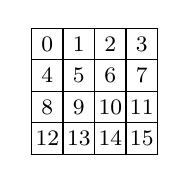
\begin{tikzpicture}[xscale=0.4,yscale=0.4]
      \footnotesize
      \foreach \i in {0,1,2,3}{
        \foreach \j in {0,1,2,3}{
          \draw (\i,\j) rectangle (\i+1,\j+1) ;
        }
      }
      \draw (.5,3.5) node {$0$};
      \draw (1.5,3.5) node {$1$};
      \draw (2.5,3.5) node {$2$};
      \draw (3.5,3.5) node {$3$};

      \draw (.5,2.5) node {$4$};
      \draw (1.5,2.5) node {$5$};
      \draw (2.5,2.5) node {$6$};
      \draw (3.5,2.5) node {$7$};

      \draw (.5,1.5) node {$8$};
      \draw (1.5,1.5) node {$9$};
      \draw (2.5,1.5) node {$10$};
      \draw (3.5,1.5) node {$11$};

      \draw (.5,.5) node {$12$};
      \draw (1.5,.5) node {$13$};
      \draw (2.5,.5) node {$14$};
      \draw (3.5,.5) node {$15$};
    \end{tikzpicture}
    \caption{\label{fig:numbering}Numbering in the FSM.}
  \end{subfigure}
  \hfill~
  
  \caption{\label{fig:notations-all}Our notations. Note that the numbering of the digits differs from the one traditionally used for the \gls{AES}.}
\end{figure}


% Leo: ce qui suit est pour qu'emacs compile bien l'article, pas touche !
%%% Local Variables:
%%% mode: latex
%%% ispell-local-dictionary: "english"
%%% TeX-master: "../main"
%%% End:







\paragraph{S-box Layer ($\subW$).}
We let $\thesbox$ be defined by its lookup table:
\begin{equation}
  \label{eq:thesbox}
  \thesbox = {\tt [1, 12, 6, 11, 14, 3, 15, 5, 10, 9, 13, 16, 7, 8, 0, 2, 4]}
\end{equation}
so that $\thesbox(0) = 1$, $\thesbox(1) = 12$, and so on. It has the following polynomial representation, and is thus of maximum degree: %\jb{il y a un $13x^{10}$  dans le polynome. C'est un $13x^{10}$ ?}\lp{oui}
\begin{equation*}
  \begin{split}
    \thesbox(x) ~=~& 1 + 4 x^{1} + 13 x^{2} + 7 x^{3} + 16 x^{4} + 15 x^{5} + 5 x^{7} + 5 x^{8} \\
    & + 11 x^{9} + 13 x^{10} + 12 x^{11} + 13 x^{12} + 15 x^{14} + x^{15}~.
  \end{split}
\end{equation*}
It was chosen by enumerating all APN permutations of $\mathbb{F}_{17}$, i.e., all permutations $A$ such that the equation $A(x+a)=A(x)+b$ has at most 2 solutions $x$ for all $a \neq 0$ and all $b$. Then, we selected $\thesbox$ among those that offer a good balance between minimizing the number of pairs $(a,b)$ for which the previous equation has exactly two solutions, and minimizing the maximum modulus of the Walsh spectrum (see Definition~\ref{def:fourier}).


\paragraph{Linear Layer ($\mixC$).} We opted for a $4 \times 4$ Maximum Distance Separable (MDS) matrix to ensure optimal diffusion. The matrix we chose is 
\begin{equation}
  \label{eq:mixmat}
  \mixmat = \left[ { \tiny
      \begin{array}{rrrr}
        2 & 1 & 1 & 1 \\
        1 & -1 &1 & -2 \\
        1 & 1 & -2 &-1 \\
        1 & -2 &-1 &1 \\
      \end{array}
    }\right]~.
   % \begin{array}{cccc}
    %  -1 & -1 & -1 & 2 \\
     % -1 & 1 & 2 & -1 \\
     % -1 & 2 & 1 & 1 \\
     % 2 & 1 & -1 & 1 \\
   % \end{array} \right]~.
\end{equation}
%We obtained it by performing an exhaustive search of all $4 \times 4$ matrices with coefficients in ${-2,-1,1,2}$ with at most one coefficient 2 or -2 in each row, and then picking one with the smallest $\ell_2$-norm for a matrix with coefficients in $\mathbb{F}_{17}$. The idea with our initial restrictions to ensure that the $\ell_2$ norm will be low as it depends on the absolute value of the coefficients.

We verified that there is no MDS matrix in  $\mathbb{F}_{17}$ with coefficients in $\{-1,1\}$ by exhaustively  testing all such matrices. As we were interested in MDS matrices with minimal $\ell_2$-norm and we were able to find during the initial experiments  matrices with a squared $\ell_2$-norm of 7, it was evident from the definition of the $\ell_2$-norm that matrices with minimal $\ell_2$-norm could not have coefficients $x$ with $|x| > 2$.  Thus, by testing all matrices with coefficients in $\{-2,-1,1,2\}$, we found a total of $30\>720$ MDS matrices with an $\ell_2$-norm of 7. We selected $\mixmat$ for its symmetries, particularly because it is its own transpose. % Among them, some matrices had a more structured form, as they could be written as 

% \begin{equation*}
%   \mixmat = \left[
%   \begin{array}{rr}
%     A & B  \\
%     B & -A 
%   \end{array} \right]~.
% \end{equation*}
% where both $A$ and $B$ are $2\times 2$ matrices. There were in total 256 matrices of this particular form and we chose $M$ randomly among them, taking into account also that $\mixmat = \mixmat^{T}$.
% (which means its linear behaviour is close to its differential behaviour). \leo{À vérifier}\ac{Cette phrase est bizarre : les branch nb et la distribution des poids sont les memes pour les deux codes si le code est MDS. Donc je ne vois pas ce que cela apporte qu'ils soient identiques.} \leo{ok, j'ai viré}


\paragraph{Filter.} The filter function $\filter$ maps $\mainField^{16}$ (i.e., the full FSM state) to a tuple $(a,b,c,d)$ in $\mainField^{4}$. As summarized in Figure~\ref{fig:filter}, we have that $a,b,c$ and $d$ correspond to the digits of the FSM state with indices 4, 6, 12, and 14 respectively (using the numbering from Figure~\ref{fig:numbering}).


\paragraph{LFSRs.} The whitening LFSR $\whitening$ and the key schedule LFSR $\pseudoKS$ are simply LFSRs over \(\F_p\) of maximum period, and have length 32 and 64 respectively. We obtain a
  maximum-period LFSR over $\mainField^w$ using the coefficients of a
  primitive polynomial as the taps.  More precisely, we used the {\tt SageMath}
  implementation of the finite field $\F_{p^w}$, which resulted in a pseudo-Conway polynomial. The output of the LFSR is taken from its last cell.

  More precisely, an LFSRs of length $\ell$ at time $t$ is a list of digits ${x^t_0, ..., x^t_{\ell-1}}$
  that is clocked as follows:
  \begin{enumerate}
  \item $x_0^{t+1} \gets - \sum_{i=0}^{\ell-1} x_i^t c_i$,
  \item $x_{i}^{t+1} \gets x_{i-1}^t$ for $0 < i < \ell$,
  \item the output is $x_{\ell-1}^t$,
  \end{enumerate}
  where $C=(c_i)_{0 \leq i < \ell}$ is the list of its taps, each being
  a digit of $\mathbb{F}_{17}$. We define $\clock{C}$ to be the function
  applying the operations above to a list ${x^t_0, ..., x^t_{\ell-1}}$
  to update it, and returning $x_{\ell-1}^t$.

  For the key schedule $\pseudoKS$, we use the following taps:
  \begin{equation*}
    \footnotesize
    \begin{split}
      C(\pseudoKS) ~=~& \{9, 4, 6, 4, 8, 6, 6, 16, 3,
                        9, 15, 12, 8, 12, 11, 4, 4, 8, 1,
                        8, 8, 9, 4, 6, 6, 7, 6, 3, \\
                      & 16, 14, 14, 6, 10, 15, 14, 13, 10, 1, 1,
                        10, 13, 11, 14, 10, 7, 4, 15, 8, 16,
                        3, 13, \\
                      & 14, 15, 16, 3, 16, 9, 3, 6,
                        12, 15, 9, 12, 3\}~,
    \end{split}
  \end{equation*}
  and for the whitening LFSR $\whitening$ we use
  \begin{equation*}
    \footnotesize
    \begin{split}
      C(\whitening) ~=~& \{8, 14, 14, 14, 1, 6, 12, 10, 14, 14,
                         14, 5, 2, 5, 6, 13, 6, 15, 14, 3, \\
                       & 13, 16, 1, 13, 9, 1, 7, 15, 13, 6,
                         14, 3\}~.
    \end{split}
  \end{equation*}


\paragraph{Master Key Processing.}
We generate the digits in $\pseudoKS$ first, and then those in $\whitening$. To generate them, we concatenate the 128-bit long master key with an IV and then a byte set to 1. The result is fed into \textsf{SHAKE128}, and the output byte stream of this primitive is used to generate digits of $\mathbb{F}_{17}$ using rejection sampling: if a byte $x$ is equal to 255, we discard it; otherwise, we generate the digit $\lfloor x / 15 \rfloor$. Since $15 \times 17 = 255$, this results in an unbiased transformation.


% Leo: ce qui suit est pour qu'emacs compile bien l'article, pas touche !
%%% Local Variables:
%%% mode: latex
%%% ispell-local-dictionary: "english"
%%% TeX-master: "main"
%%% End:



